\section{Durchführung}
\label{sec:Durchführung}

\subsection{Kennlinienschar der Hochvakuumdiode}
Durch Variation der Heizstromstärke wird eine Kennlinienschar 
einer Hochvakkumdiode aus fünf Kennlinien erstellt.
Dabei wird die Heizstromstärke $I_\text{H}$ auf $\num{2}$
bis $\SI{2.4}{\ampere}$ eingestellt.
Die Heizspannung $V_\text{H}$ kann jeweils abgelesen werden.
Die Anodenspannung $V_\text{A}$ wird jeweils variiert.
Dabei können die zugehörigen Werte des Anodenstroms $I_\text{A}$
abgelesen werden. Es wird die Schaltung aus Abb. \ref{fig:a}
verwendet.
%Daraus wird der Sättigungsstrom $I_S$ abgelesen. 
\begin{figure}
    \centering
    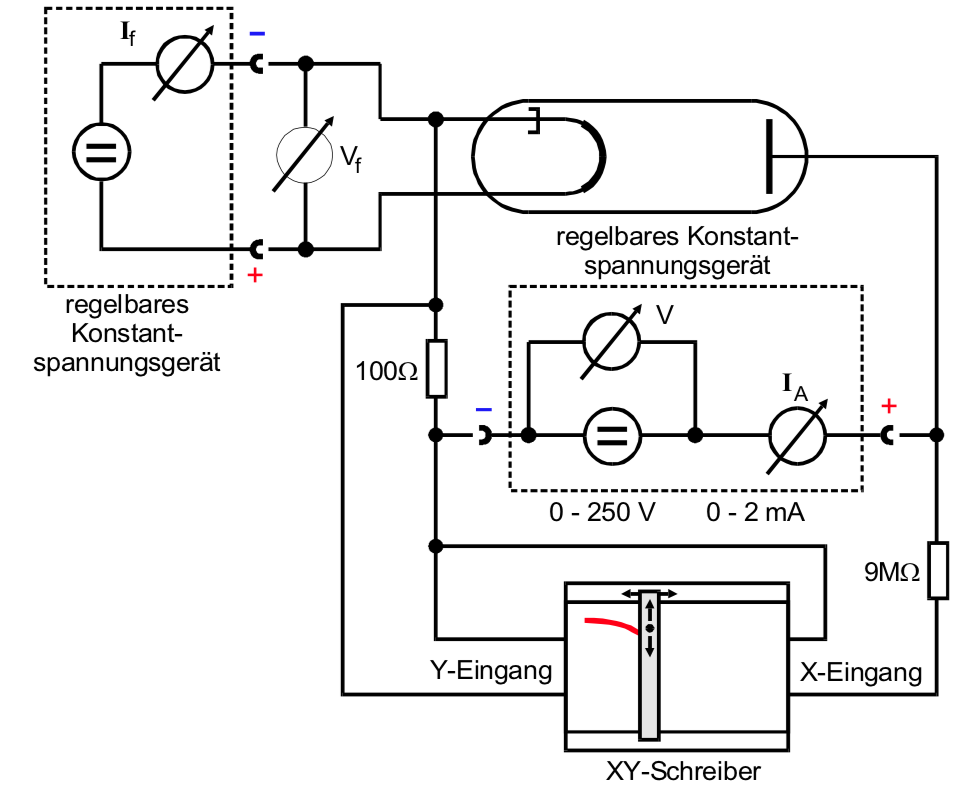
\includegraphics[width=12cm, height=9cm]{build/a.png}
    \caption{Schaltung zur Messung der Kennlinien der Hochvakuumdiode. \cite{V504}}
    \label{fig:a}
\end{figure}

\subsection{Anlaufstromgebiet der Diode}
%Es wird versucht für die maximal mögliche Heizleistung den 
%ungefähren Gültigkeitsbereich des Langmuir-Schottkyschen 
%Raumladungsgesetzes zu finden. 
%Aus den gemessenen Wertepaaren wird der Exponent der Strom-
%Spannungsbeziehung festgestellt.

Für die maximal mögliche Heizleistung wird das 
Anlaufstromgebiet der Diode untersucht.
Dafür wird die in Abb. \ref{fig:c} gezeigte Schaltung
nachgebaut. Bei der maximalen Stromstärke von 
$I_\text{H} = \SI{2.4}{\ampere}$ wird wieder für variierende
Anodenspannungen $V_\text{A}$ im Bereich von $\num{0}$ bis
$\SI{250}{\volt}$ die Anodenstromstärke $I_\text{A}$ abgelesen.
%ist das richtig?
\begin{figure}
    \centering
    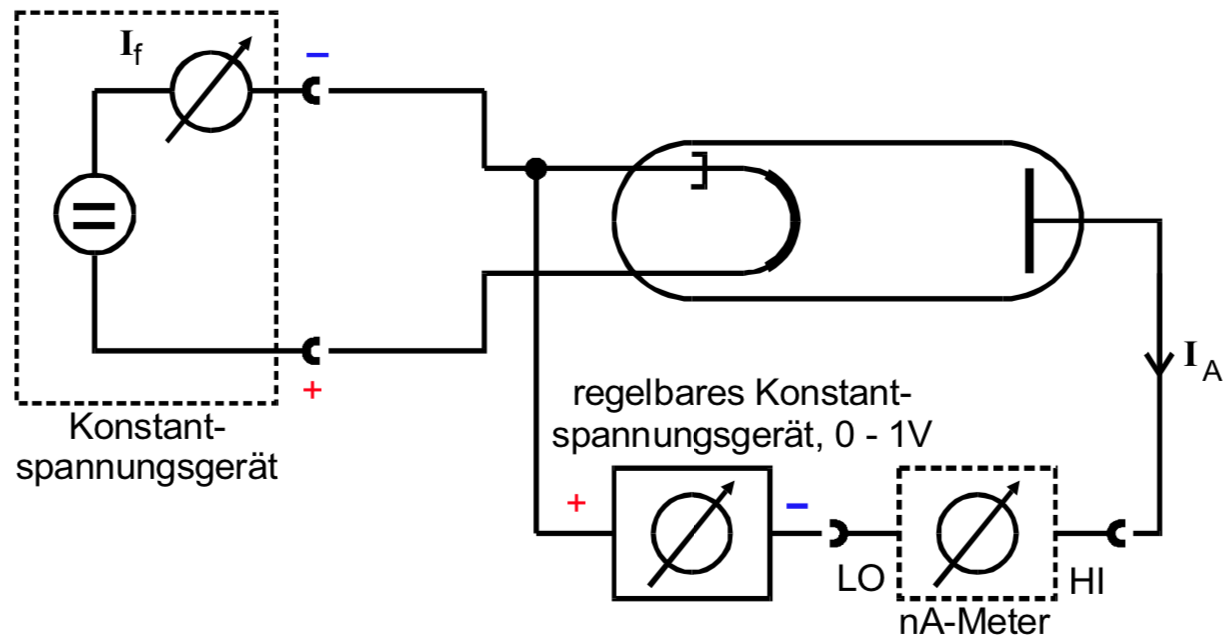
\includegraphics[width=12cm, height=7cm]{build/c.png}
    \caption{Schaltung zur Messung des Anlaufstromgebiets. \cite{V504}}
    \label{fig:c}
\end{figure}

%und die Kathodentemperatur T bestimmt. 


%Aus einer Leistungsbilanz des Heizstromkreises wird die 
%Kathodentemperatur bei den am Anfang verwendeten 
%Heizleistungen abgeschätzt. 

%Aus den Wertepaaren $T$ und $I_S$ wird die Austrittsarbeit für 
%das Kathodenmaterial berechnet. 
